\documentclass[conference]{IEEEtran}
\IEEEoverridecommandlockouts

\usepackage[spanish,es-noshorthands]{babel}
\usepackage[utf8]{inputenc}
\usepackage[T1]{fontenc}
\usepackage{cite}
\usepackage{amsmath,amssymb,amsfonts}
\usepackage{graphicx}
\usepackage{textcomp}
\usepackage{xcolor}
\usepackage{booktabs}
\usepackage{multirow}
\usepackage{url}
\usepackage{microtype}
\usepackage{caption}
\captionsetup{font=footnotesize}

\def\BibTeX{{\rm B\kern-.05em{\sc i\kern-.025em b}\kern-.08em
    T\kern-.1667em\lower.7ex\hbox{E}\kern-.125emX}}

\begin{document}

\title{Análisis de la Demanda Horaria en un Sistema de Bicicletas Compartidas: Un Enfoque de Analítica de Datos y Modelos Predictivos}

\author{
\IEEEauthorblockN{David Delgado -- Ingeniero de Datos}
\IEEEauthorblockA{\textit{Facultad de Ingeniería de Sistemas Computacionales} \\
\textit{Universidad Tecnológica de Panamá}\\
Panamá, Panamá \\
[contacto omitido]}
\and
\IEEEauthorblockN{Jeshuath Hernández -- Analista de Datos}
\IEEEauthorblockA{\textit{Facultad de Ingeniería de Sistemas Computacionales} \\
\textit{Universidad Tecnológica de Panamá}\\
Panamá, Panamá \\
[contacto omitido]}
\and
\IEEEauthorblockN{Johan Cerrud -- Científico de Datos}
\IEEEauthorblockA{\textit{Facultad de Ingeniería de Sistemas Computacionales} \\
\textit{Universidad Tecnológica de Panamá}\\
Panamá, Panamá \\
[contacto omitido]}
\and
\IEEEauthorblockN{Giovanny Arpaia -- Ingeniero de ML}
\IEEEauthorblockA{\textit{Facultad de Ingeniería de Sistemas Computacionales} \\
\textit{Universidad Tecnológica de Panamá}\\
Panamá, Panamá \\
[contacto omitido]}
}

\maketitle

\begin{abstract}
Este artículo resume el desarrollo del proyecto final del curso de Análisis de Datos y Toma de Decisiones en Computación de la Universidad Tecnológica de Panamá, aplicado al conjunto de datos \textit{Bike Sharing Dataset} (registro horario, \texttt{hour.csv}) del sistema de bicicletas compartidas Capital Bikeshare de Washington D.C. Se realizó un análisis exploratorio completo, un estudio de correlación entre variables climáticas, temporales y de demanda, y el entrenamiento de modelos de clasificación y regresión para predecir el nivel y la magnitud de la demanda horaria. El mejor modelo de clasificación (Random Forest) alcanzó una exactitud de prueba de 0.878, mientras que el mejor modelo de regresión (Random Forest Regressor) obtuvo un coeficiente de determinación de prueba de 0.945. Los resultados se integraron en un dashboard interactivo desarrollado en Microsoft Power BI. Se identificaron patrones horarios claramente diferenciados entre días laborales y fines de semana, así como una relación relevante entre condiciones climáticas y volumen de alquileres.
\end{abstract}

\begin{IEEEkeywords}
analítica de datos, aprendizaje automático, bicicletas compartidas, Random Forest, series de tiempo, Power BI, ciencia de datos
\end{IEEEkeywords}

\section{Introducción}

Los sistemas de bicicletas compartidas generan grandes volúmenes de datos operativos que pueden analizarse para comprender los patrones de movilidad urbana y anticipar la demanda del servicio. Esta información es valiosa tanto para la planificación de flotas como para la optimización de la disponibilidad de bicicletas en las estaciones a lo largo del día.

Este proyecto utiliza la Analítica de Datos para responder la siguiente pregunta principal: \textbf{¿en qué horas del día se concentra la mayor demanda de bicicletas y cómo varía ese patrón entre días laborables y fines de semana?} A partir de esta pregunta se derivaron las siguientes subpreguntas:

\begin{itemize}
\item ¿Cuáles son las horas pico de uso durante un día laboral frente a un fin de semana?
\item ¿El comportamiento horario de los usuarios casuales difiere del de los usuarios registrados?
\item ¿Las condiciones climáticas afectan la demanda en ciertas horas más que en otras?
\item ¿Existen franjas horarias con demanda consistentemente baja, independientemente del día?
\end{itemize}

Para responder estas preguntas se desarrolló un flujo completo de trabajo con datos: preparación y limpieza, análisis exploratorio y de correlación, entrenamiento de modelos predictivos de clasificación y regresión, y despliegue de un dashboard interactivo que resume los hallazgos y permite explorar el comportamiento de la demanda de forma dinámica.

\section{Materiales y Métodos}

\subsection{Descripción del dataset}

Se utilizó el \textit{Bike Sharing Dataset}, publicado en el repositorio UCI Machine Learning Repository y construido originalmente por Fanaee-T y Gama a partir de los registros abiertos del sistema Capital Bikeshare de Washington D.C.\ \cite{fanaee2014}. De las dos tablas que ofrece el repositorio (\texttt{day.csv} y \texttt{hour.csv}) se seleccionó \texttt{hour.csv}, ya que agrega la demanda a nivel horario y permite responder directamente la pregunta sobre los patrones de uso a lo largo del día.

El dataset contiene \textbf{17{,}379 observaciones} y \textbf{17 variables}, correspondientes al periodo comprendido entre el 1 de enero de 2011 y el 31 de diciembre de 2012. Cada fila representa una hora e incluye variables temporales (\texttt{season}, \texttt{yr}, \texttt{mnth}, \texttt{hr}, \texttt{holiday}, \texttt{weekday}, \texttt{workingday}), climáticas (\texttt{weathersit}, \texttt{temp}, \texttt{atemp}, \texttt{hum}, \texttt{windspeed}) y de demanda (\texttt{casual}, \texttt{registered}, \texttt{cnt}, donde \texttt{cnt = casual + registered}).

\subsection{Herramientas y librerías}

El procesamiento, análisis exploratorio y modelado se desarrolló en Python, utilizando las siguientes librerías: \textbf{pandas} y \textbf{numpy} para manipulación de datos; \textbf{matplotlib} y \textbf{seaborn} para visualización \cite{hunter2007,waskom2021}; \textbf{missingno} y \textbf{upsetplot} para el análisis de valores faltantes \cite{bilogur2018,lex2014}; y \textbf{scikit-learn} para el entrenamiento y evaluación de los modelos predictivos \cite{pedregosa2011}, con \textbf{joblib} para la serialización del modelo final. El dashboard de resultados se construyó con \textbf{Microsoft Power BI Desktop} y se publicó mediante \textbf{Power BI Service} \cite{powerbi2026}.

\subsection{Metodología}

Como primer paso se realizó un análisis preliminar del dataset (tipos de dato, valores únicos, medidas de tendencia central y de dispersión) y una revisión exhaustiva de valores faltantes mediante tablas resumen, \texttt{missingno.matrix}, \texttt{missingno.bar} y \texttt{UpSetPlot}. Al no encontrarse valores faltantes, duplicados, columnas vacías ni valores infinitos, no fue necesario aplicar el procedimiento de eliminación (variables con más de 250 valores faltantes) ni de imputación previsto en la guía del proyecto; el procedimiento se dejó documentado y programado en el notebook para evidenciar su cumplimiento.

Posteriormente se realizaron dos análisis de correlación (Pearson y Spearman) entre las variables temporales, climáticas y de demanda, considerando que \texttt{casual} y \texttt{registered} son componentes directos de \texttt{cnt} y por lo tanto presentan correlaciones naturalmente altas con dicha variable.

Para el modelado predictivo se definieron dos tareas:

\begin{itemize}
\item \textbf{Clasificación}: se construyó la variable categórica \texttt{nivel\_demanda} (Baja / Media / Alta) mediante terciles de \texttt{cnt}, y se entrenaron un \textit{Random Forest Classifier} y un \textit{K-Nearest Neighbors Classifier} (con estandarización de variables).
\item \textbf{Regresión}: se utilizó \texttt{cnt} como variable objetivo continua, entrenando un \textit{Random Forest Regressor} y un \textit{Support Vector Regressor} (SVR, kernel RBF, con estandarización de variables).
\end{itemize}

En ambos casos se utilizaron como predictoras las 12 variables temporales y climáticas (\texttt{season}, \texttt{yr}, \texttt{mnth}, \texttt{hr}, \texttt{holiday}, \texttt{weekday}, \texttt{workingday}, \texttt{weathersit}, \texttt{temp}, \texttt{atemp}, \texttt{hum}, \texttt{windspeed}), excluyendo deliberadamente \texttt{casual} y \texttt{registered} por ser componentes directos de la variable objetivo (fuga de información). Se aplicó una partición 80/20 para entrenamiento y prueba (estratificada en el caso de clasificación), y se calcularon exactitud (\textit{accuracy}) y matriz de confusión para los modelos de clasificación, y coeficiente de determinación ($R^2$), RMSE y MAE para los modelos de regresión, en ambos subconjuntos. El modelo de regresión con mejor desempeño se serializó con \texttt{joblib} para su uso posterior en el dashboard.

\subsection{Mapa interactivo de distritos de Panamá}

\textcolor{red}{\textbf{[PENDIENTE -- ver nota para el equipo].}} La guía del proyecto solicita, como contenido mínimo del dashboard, un mapa interactivo a nivel de distritos de Panamá construido con \textbf{GeoPandas}, utilizando límites geográficos de geoBoundaries y al menos una variable sociodemográfica del Mapa Interactivo del INEC (MapI). Esta sección debe completarse con: (a) la variable sociodemográfica seleccionada, (b) la fuente exacta de los límites distritales utilizados y (c) el rol responsable de su construcción, una vez el equipo defina e incorpore este componente al dashboard.

\section{Resultados}

\subsection{Análisis exploratorio}

La variable \texttt{cnt} (total de bicicletas alquiladas por hora) presenta una media de 189.46, mediana de 142, moda de 5, primer cuartil de 40 y tercer cuartil de 281, con una desviación estándar de 181.39. El coeficiente de asimetría (1.28) confirma un sesgo positivo: la mayoría de las horas registran una demanda baja o moderada, mientras que un número menor de horas concentra picos muy altos de alquiler (Fig.~\ref{fig:distribucion}).

\begin{figure}[!t]
\centering
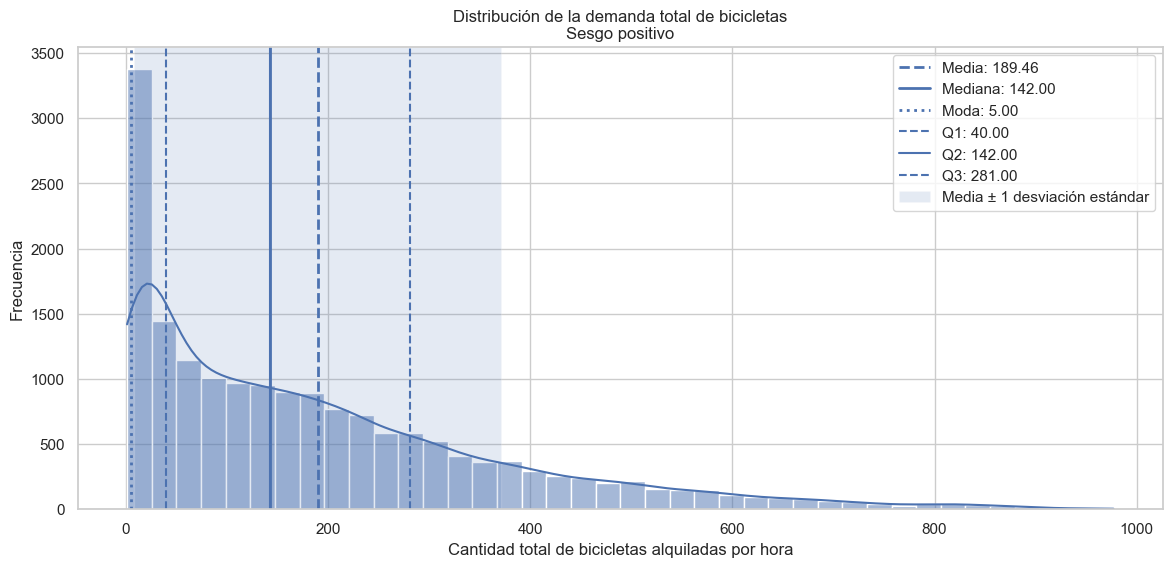
\includegraphics[width=\linewidth]{figs/fig_distribucion_cnt.png}
\caption{Distribución de la demanda total de bicicletas por hora, con media, mediana, moda y cuartiles.}
\label{fig:distribucion}
\end{figure}

Al comparar el promedio de demanda por hora entre días laborales y fines de semana o feriados (Fig.~\ref{fig:demanda_hora}), se observa un patrón claramente bimodal en los días laborales, con picos asociados a los horarios de entrada y salida del trabajo: las horas de mayor demanda son las \textbf{17h (525.3), 18h (492.2), 8h (477.0), 19h (348.4) y 16h (293.1)}. En cambio, durante fines de semana o feriados el patrón es unimodal y centrado en el mediodía, con las horas de mayor demanda ubicadas en \textbf{13h (372.7), 12h (366.3), 14h (364.6), 15h (358.8) y 16h (352.7)}. Las horas de menor demanda promedio, en ambos tipos de día, se concentran en la madrugada: \textbf{4h (6.4), 3h (11.7), 5h (19.9), 2h (22.9) y 1h (33.4)}, todas por debajo del umbral de baja demanda (percentil 25 del promedio horario, 70.51 bicicletas).

\begin{figure}[!t]
\centering
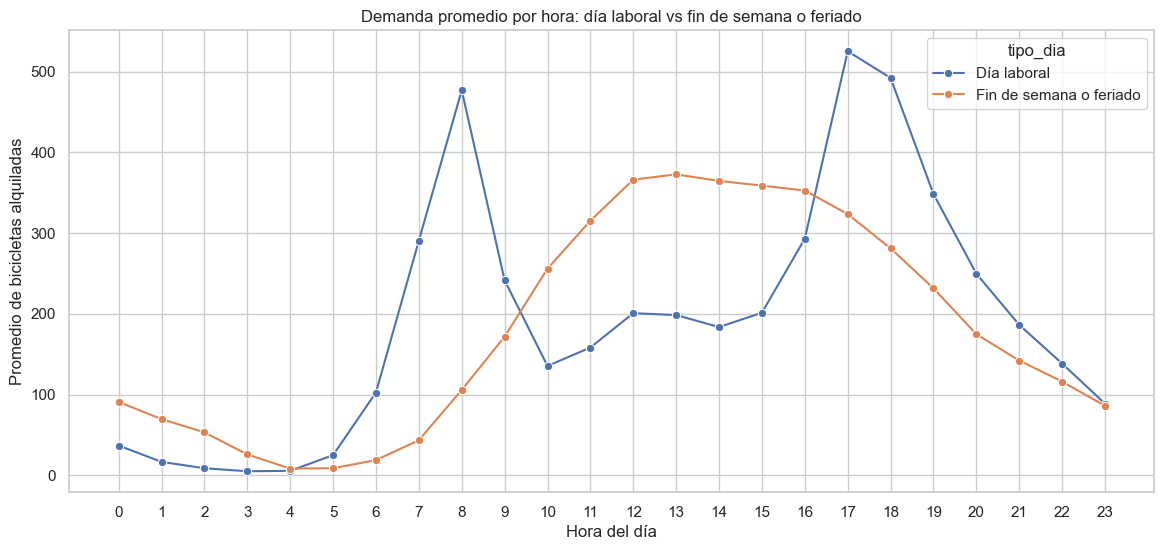
\includegraphics[width=\linewidth]{figs/fig_demanda_hora_tipo.png}
\caption{Demanda promedio por hora: día laboral vs. fin de semana o feriado.}
\label{fig:demanda_hora}
\end{figure}

El comportamiento horario también difiere entre tipos de usuario (Fig.~\ref{fig:casual_registrado}): los usuarios \textbf{registrados} muestran el mismo patrón bimodal ligado a los desplazamientos laborales, mientras que los usuarios \textbf{casuales} presentan una curva más suave, concentrada en horas de la tarde, coherente con un uso recreativo más que de traslado diario.

\begin{figure}[!t]
\centering
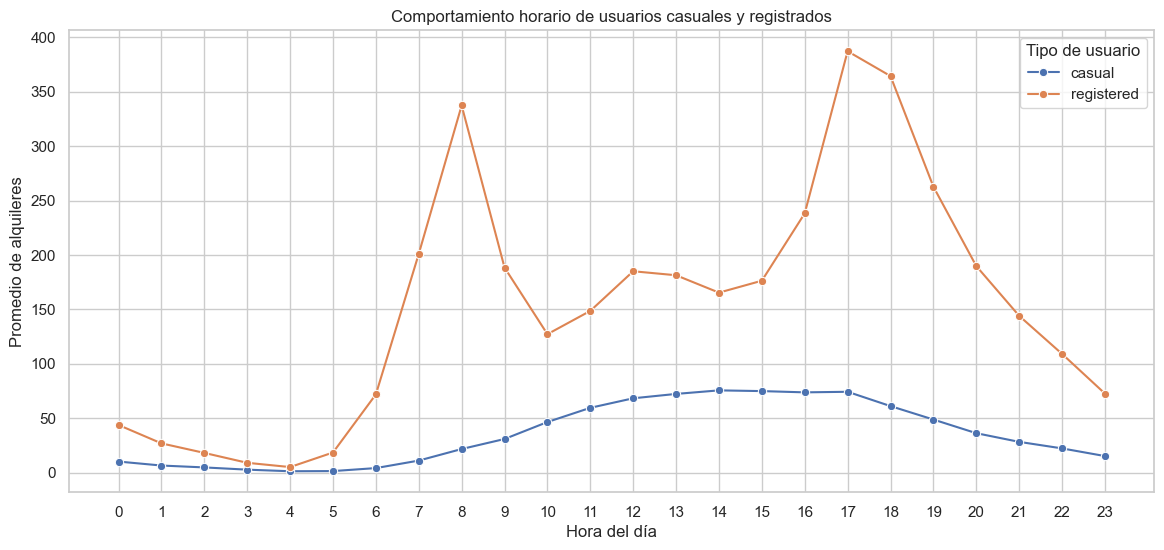
\includegraphics[width=\linewidth]{figs/fig_casual_registrado.png}
\caption{Comportamiento horario promedio de usuarios casuales y registrados.}
\label{fig:casual_registrado}
\end{figure}

Respecto al efecto del clima (Fig.~\ref{fig:clima} y Fig.~\ref{fig:heatmap}), la demanda promedio por hora es sistemáticamente menor en condiciones de lluvia o nieve, en comparación con condiciones despejadas o de neblina, y el mapa de calor por día de la semana y hora confirma que el patrón bimodal entre semana y el patrón centrado al mediodía en fines de semana se mantiene de forma consistente a lo largo de todo el periodo analizado.

\begin{figure*}[!t]
\centering
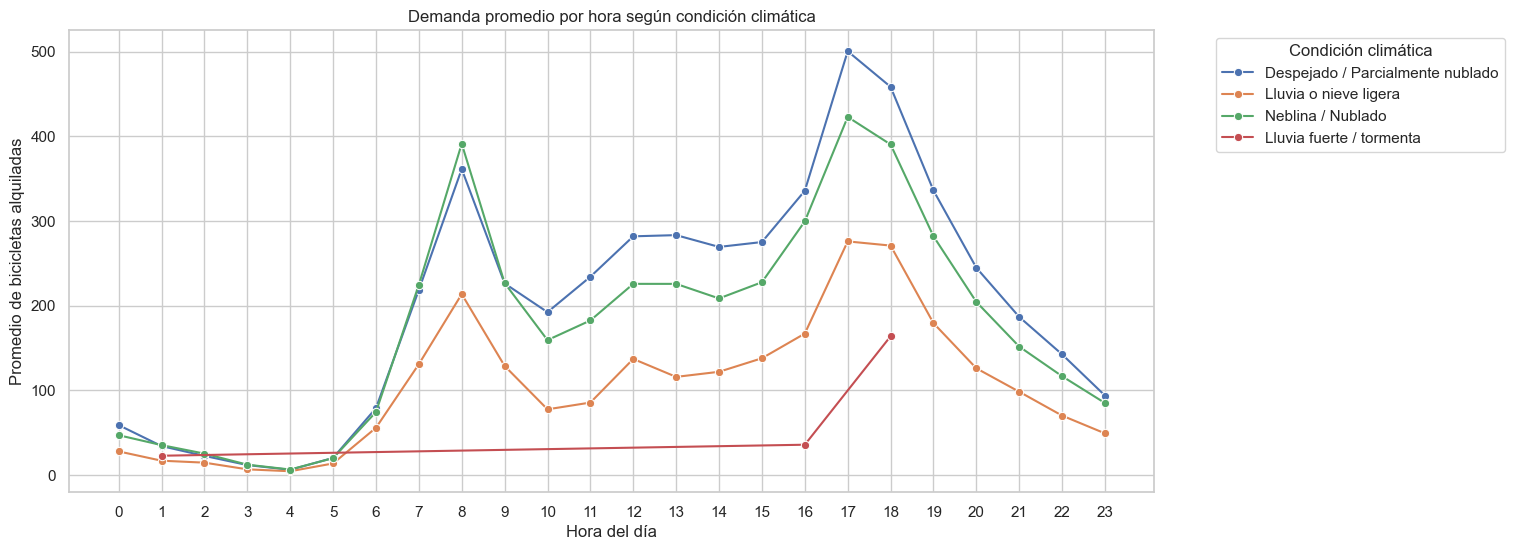
\includegraphics[width=0.85\textwidth]{figs/fig_clima.png}
\caption{Demanda promedio por hora según condición climática.}
\label{fig:clima}
\end{figure*}

\begin{figure*}[!t]
\centering
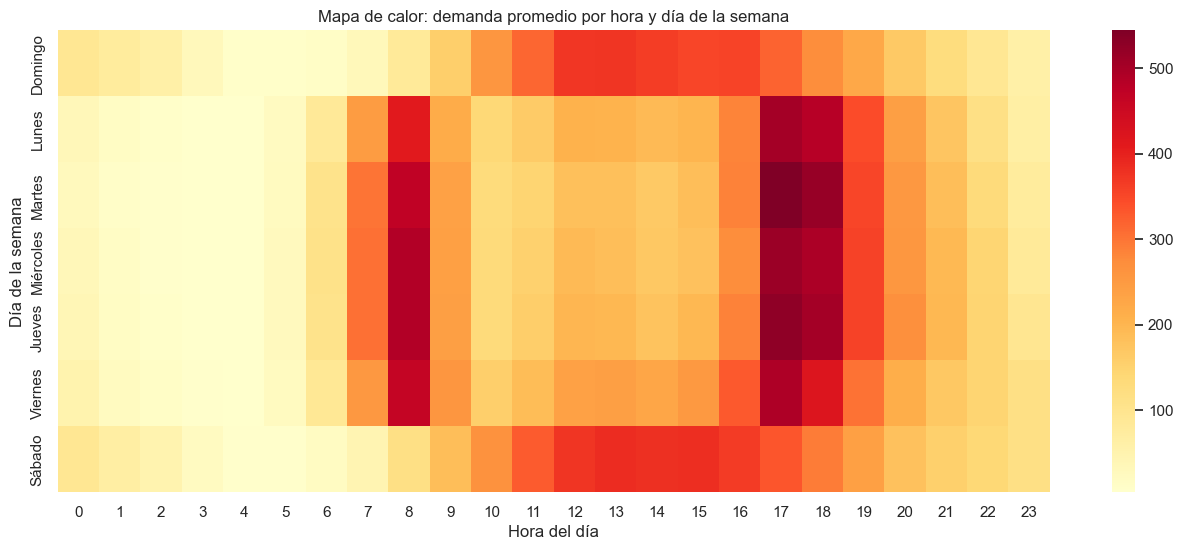
\includegraphics[width=0.85\textwidth]{figs/fig_heatmap.png}
\caption{Mapa de calor de la demanda promedio por hora y día de la semana.}
\label{fig:heatmap}
\end{figure*}

\subsection{Análisis de correlación}

La Tabla~\ref{tab:correlacion} resume los coeficientes de correlación de Pearson y Spearman entre cada variable y \texttt{cnt}. Como es de esperarse, \texttt{registered} y \texttt{casual} muestran las correlaciones más altas por ser componentes directos de la variable objetivo. Entre las variables verdaderamente predictoras, la temperatura (\texttt{temp}, \texttt{atemp}) y la hora del día (\texttt{hr}) presentan las correlaciones positivas más fuertes, mientras que la humedad (\texttt{hum}) es la variable con correlación negativa más marcada. La condición climática (\texttt{weathersit}) también se correlaciona negativamente con la demanda.

\begin{table}[!t]
\centering
\caption{Correlación de cada variable con la demanda total (\texttt{cnt})}
\label{tab:correlacion}
\begin{tabular}{lrr}
\toprule
\textbf{Variable} & \textbf{Pearson} & \textbf{Spearman} \\
\midrule
registered   & 0.972  & 0.989 \\
casual       & 0.695  & 0.851 \\
temp         & 0.405  & 0.423 \\
atemp        & 0.401  & 0.423 \\
hr           & 0.394  & 0.511 \\
yr           & 0.250  & 0.208 \\
season       & 0.178  & 0.185 \\
mnth         & 0.121  & 0.126 \\
windspeed    & 0.093  & 0.127 \\
workingday   & 0.030  & 0.021 \\
weekday      & 0.027  & 0.030 \\
holiday      & -0.031 & -0.030 \\
weathersit   & -0.142 & -0.126 \\
hum          & -0.323 & -0.360 \\
\bottomrule
\end{tabular}
\end{table}

\begin{figure*}[!t]
\centering
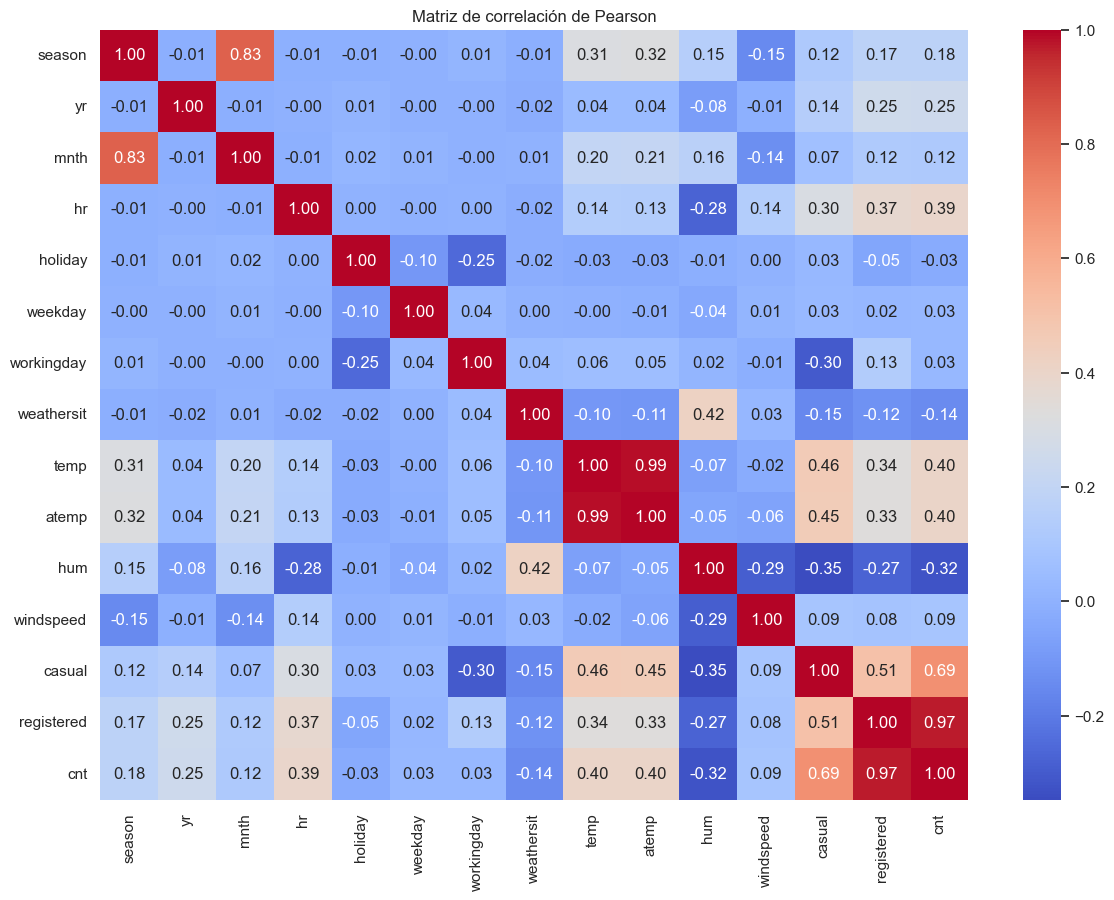
\includegraphics[width=0.7\textwidth]{figs/fig_pearson.png}
\caption{Matriz de correlación de Pearson entre las variables del dataset.}
\label{fig:pearson}
\end{figure*}

\subsection{Modelos de clasificación}

Para la tarea de clasificación se predijo el nivel de demanda (\texttt{Baja}/\texttt{Media}/\texttt{Alta}, con 5{,}797, 5{,}823 y 5{,}759 observaciones respectivamente) usando un \textit{Random Forest Classifier} y un \textit{KNN Classifier} ($k=7$). La Tabla~\ref{tab:clasificacion} resume la exactitud obtenida en entrenamiento y prueba.

\begin{table}[!t]
\centering
\caption{Resultados de los modelos de clasificación}
\label{tab:clasificacion}
\begin{tabular}{lrr}
\toprule
\textbf{Modelo} & \textbf{Accuracy train} & \textbf{Accuracy test} \\
\midrule
Random Forest Classifier & 1.000 & \textbf{0.878} \\
KNN Classifier ($k=7$)   & 0.804 & 0.729 \\
\bottomrule
\end{tabular}
\end{table}

El \textit{Random Forest Classifier} obtuvo el mejor desempeño en prueba (0.878), aunque su exactitud perfecta en entrenamiento (1.000) evidencia sobreajuste esperado en este tipo de modelos de árboles sin restricción de profundidad. El \textit{KNN} generalizó de forma más conservadora, con una brecha menor entre entrenamiento y prueba. La Fig.~\ref{fig:confusion} presenta las matrices de confusión de ambos modelos en entrenamiento y prueba.

\begin{figure*}[!t]
\centering
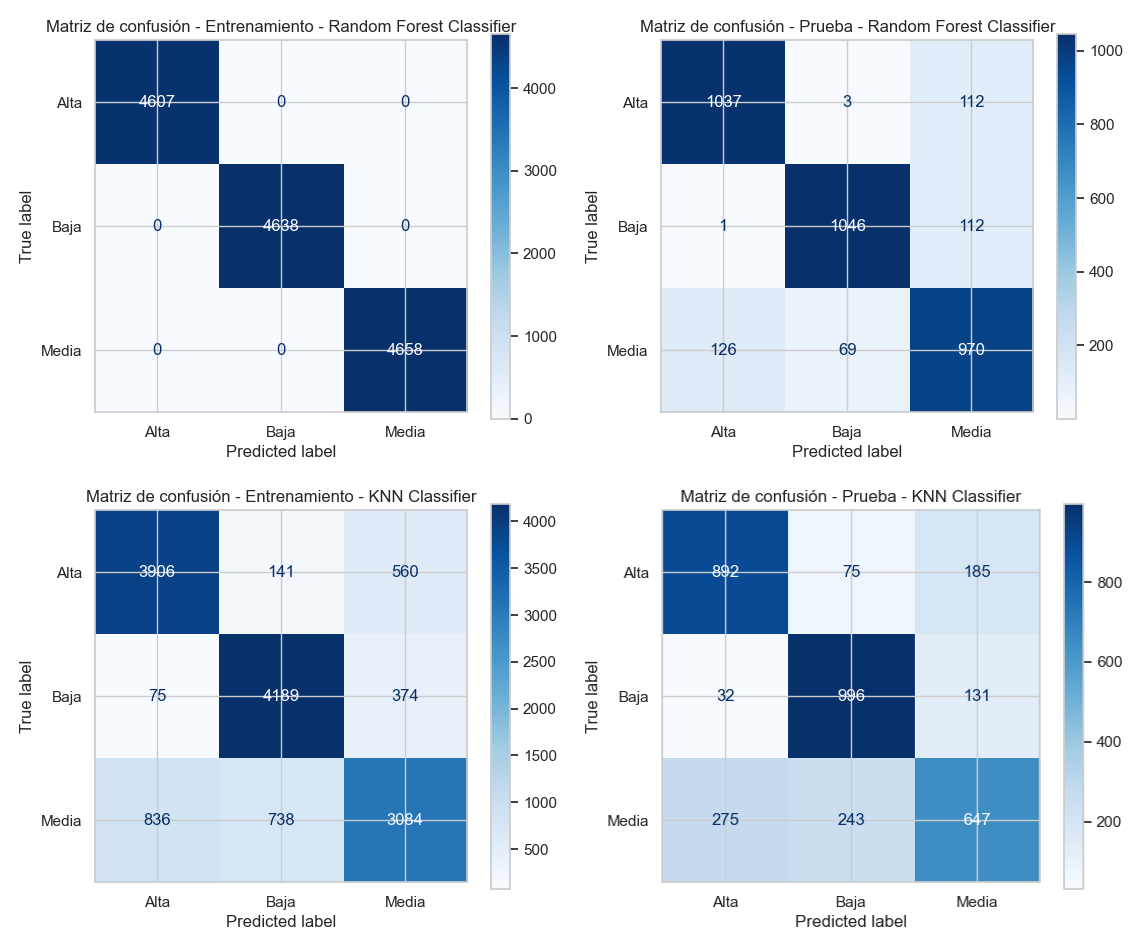
\includegraphics[width=0.75\textwidth]{figs/fig_matrices_confusion.png}
\caption{Matrices de confusión de los modelos de clasificación. Fila superior: Random Forest (entrenamiento / prueba). Fila inferior: KNN (entrenamiento / prueba).}
\label{fig:confusion}
\end{figure*}

\subsection{Modelos de regresión}

Para la tarea de regresión se predijo directamente \texttt{cnt} usando un \textit{Random Forest Regressor} y un \textit{SVR} (kernel RBF). La Tabla~\ref{tab:regresion} resume el coeficiente $R^2$, el RMSE y el MAE obtenidos en prueba.

\begin{table}[!t]
\centering
\caption{Resultados de los modelos de regresión}
\label{tab:regresion}
\begin{tabular}{lrrrr}
\toprule
\textbf{Modelo} & \textbf{$R^2$ train} & \textbf{$R^2$ test} & \textbf{RMSE} & \textbf{MAE} \\
\midrule
Random Forest Regressor & 0.992 & \textbf{0.945} & 41.80 & 24.72 \\
SVR (RBF)                & 0.604 & 0.597 & 112.92 & 67.94 \\
\bottomrule
\end{tabular}
\end{table}

El \textit{Random Forest Regressor} superó ampliamente al SVR, explicando el 94.5\% de la varianza de la demanda en el conjunto de prueba, con un error absoluto medio de aproximadamente 24.7 bicicletas por hora. Este fue el modelo seleccionado y serializado para su uso en el dashboard interactivo. La Fig.~\ref{fig:regresion} compara los valores reales contra los predichos por ambos modelos.

\begin{figure*}[!t]
\centering
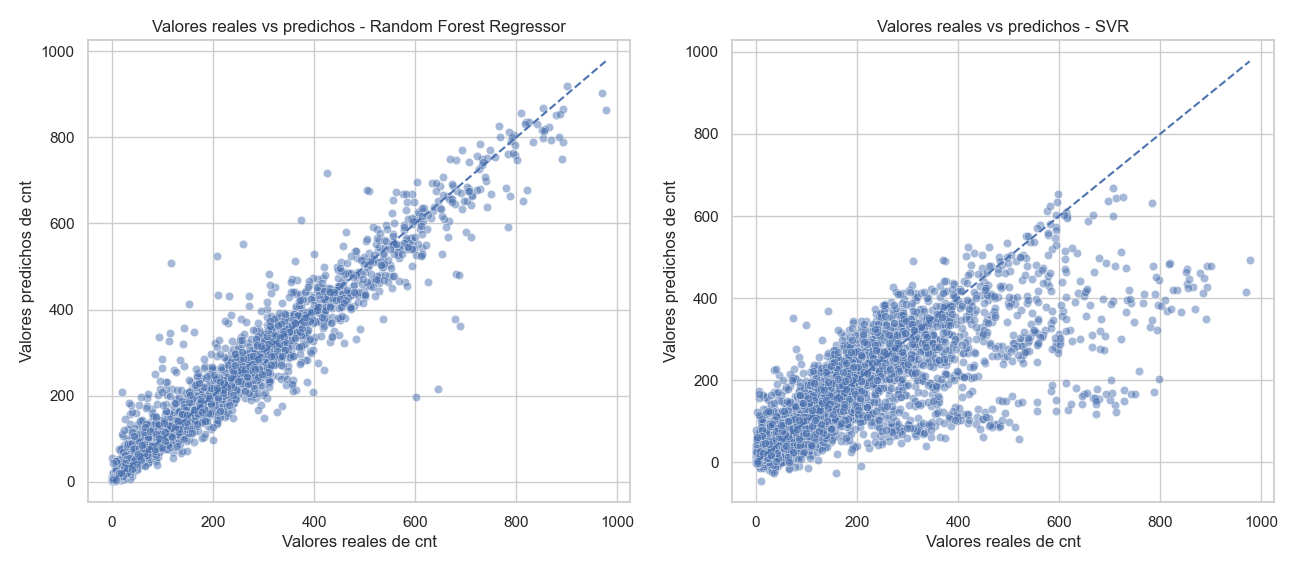
\includegraphics[width=0.85\textwidth]{figs/fig_regresion_scatter.png}
\caption{Valores reales vs.\ predichos en el conjunto de prueba: Random Forest Regressor (izquierda) y SVR (derecha).}
\label{fig:regresion}
\end{figure*}

\subsection{Dashboard interactivo y publicación}

Los resultados del análisis se integraron en un dashboard desarrollado en \textbf{Microsoft Power BI Desktop}, organizado en cinco páginas:

\begin{itemize}
\item \textbf{Página 1 -- Resumen general}: tarjetas KPI (total de bicicletas, demanda promedio, demanda máxima y total de registros), gráfico de líneas de demanda promedio por hora y tipo de día, y cuatro segmentadores interactivos (año, estación, tipo de día y condición climática).
\item \textbf{Página 2 -- Usuarios casuales vs.\ registrados}: gráficos de líneas del comportamiento horario de cada tipo de usuario y un gráfico de columnas apiladas por hora.
\item \textbf{Página 3 -- Efecto del clima}: demanda promedio por hora según condición climática y un gráfico de dispersión entre sensación térmica y demanda.
\item \textbf{Página 4 -- Evaluación de modelos predictivos}: tarjetas con la mejor exactitud de clasificación, el mejor $R^2$ y el menor RMSE de regresión, y el modelo utilizado; tablas y gráficos comparativos de los modelos de clasificación y regresión; y una tabla dinámica de la matriz de confusión filtrable por modelo mediante un segmentador.
\item \textbf{Página 5 -- Distribución y calidad de datos}: imágenes del análisis de valores faltantes y de la distribución de la variable \texttt{cnt}, exportadas directamente del notebook.
\end{itemize}

Todas las páginas incorporan segmentadores y controles que reaccionan de forma interactiva a las selecciones del usuario, filtrando de manera cruzada las visualizaciones de cada página.

\textcolor{red}{\textbf{[PENDIENTE -- completar con datos reales del equipo antes de entregar]:}} el dashboard se publicó en \underline{\hspace{2.2cm}} (indicar si fue mediante \textit{Publicar en la Web} de Power BI, un enlace de Power BI Service, u otra plataforma), cuyo requisito de acceso fue \underline{\hspace{2.2cm}} (p.\ ej., cuenta institucional, enlace público, licencia Pro/PPU). El enlace público al dashboard es: \url{https://[COMPLETAR-ENLACE-DEL-DASHBOARD]}. Asimismo, debe confirmarse si el control de la Página 4 permite ingresar una instancia arbitraria para obtener una predicción en vivo del modelo de regresión, tal como lo exige la guía del proyecto, o si opera sobre un conjunto predefinido de escenarios.

\section{Conclusiones}

Los datos analizados muestran que la demanda de bicicletas compartidas responde principalmente a un patrón de movilidad urbana: en días laborales existen dos picos claros de demanda asociados a la entrada (8h) y salida (17h--18h) del trabajo, mientras que en fines de semana y feriados la demanda se concentra alrededor del mediodía y las primeras horas de la tarde (12h--15h). Los usuarios registrados explican en gran medida el patrón bimodal entre semana, mientras que los usuarios casuales muestran un uso más recreativo. Las condiciones climáticas adversas (lluvia o nieve) reducen consistentemente la demanda en todas las franjas horarias, y las horas de la madrugada (1h--5h) presentan una demanda baja de forma sistemática, independientemente del día. El modelo de Random Forest, tanto en su versión de clasificación como de regresión, demostró ser el más adecuado para modelar esta relación, con una capacidad predictiva sustancialmente mayor que KNN o SVR sobre las mismas variables.

\textit{Conclusión del Ingeniero de Datos -- David Delgado:} La verificación exhaustiva del dataset confirmó que las 17{,}379 observaciones no presentan valores faltantes, duplicados ni registros infinitos, lo cual se validó mediante tablas resumen, \texttt{missingno.matrix} y \texttt{UpSetPlot}. Esto permitió omitir el proceso de imputación previsto en la guía y entregar al resto del equipo un conjunto de datos íntegro y con tipos de variable correctamente definidos (categóricas, temporales y continuas), acelerando las etapas posteriores de análisis y modelado.

\textit{Conclusión de la Analista de Datos -- Jeshuath Hernández:} El análisis exploratorio y de correlación permitió responder directamente la pregunta inicial del proyecto: la demanda de bicicletas sigue un patrón bimodal en días laborales (picos a las 8h y entre 17h-18h) y un patrón unimodal centrado en el mediodía durante fines de semana y feriados. La hora del día y la temperatura resultaron ser las variables con mayor correlación positiva con la demanda, mientras que la humedad y las condiciones climáticas adversas se correlacionan negativamente, evidenciando que el comportamiento de los usuarios está fuertemente ligado tanto a la rutina laboral como al clima.

\textit{Conclusión del Científico de Datos -- Johan Cerrud:} Al comparar los algoritmos entrenados, el Random Forest superó de forma consistente tanto a KNN (en clasificación) como a SVR (en regresión), alcanzando una exactitud de prueba de 0.878 y un $R^2$ de prueba de 0.945 respectivamente. La exactitud perfecta del Random Forest en entrenamiento (1.000) evidenció un sobreajuste esperado en modelos de árboles sin restricción de profundidad, pero su desempeño en el conjunto de prueba lo confirmó como el modelo más robusto para capturar las relaciones no lineales entre las variables temporales/climáticas y la demanda, por lo que fue el seleccionado para ambas tareas.

\textit{Conclusión del Ingeniero de ML -- Giovanny Arpaia:} El modelo de Random Forest Regressor, por ser el de mejor desempeño, fue serializado con \texttt{joblib} e integrado en el dashboard desarrollado en Microsoft Power BI, junto con los resultados de clasificación, correlación y exploración generados por el resto del equipo. Este proceso de despliegue permitió consolidar en una sola herramienta interactiva los hallazgos de todos los roles, facilitando su exploración por parte de usuarios sin conocimientos técnicos en ciencia de datos.

\begin{thebibliography}{00}
\bibitem{fanaee2014} H. Fanaee-T and J. Gama, ``Event labeling combining ensemble detectors and background knowledge,'' \textit{Progress in Artificial Intelligence}, vol.~2, no.~2--3, pp.~113--127, 2014.
\bibitem{pedregosa2011} F. Pedregosa \textit{et al.}, ``Scikit-learn: Machine learning in Python,'' \textit{Journal of Machine Learning Research}, vol.~12, pp.~2825--2830, 2011.
\bibitem{waskom2021} M. L. Waskom, ``seaborn: statistical data visualization,'' \textit{Journal of Open Source Software}, vol.~6, no.~60, p.~3021, 2021.
\bibitem{hunter2007} J. D. Hunter, ``Matplotlib: A 2D graphics environment,'' \textit{Computing in Science \& Engineering}, vol.~9, no.~3, pp.~90--95, 2007.
\bibitem{bilogur2018} A. Bilogur, ``Missingno: a missing data visualization suite,'' \textit{Journal of Open Source Software}, vol.~3, no.~22, p.~547, 2018.
\bibitem{lex2014} A. Lex, N. Gehlenborg, H. Strobelt, R. Vuillemot, and H. Pfister, ``UpSet: Visualization of intersecting sets,'' \textit{IEEE Transactions on Visualization and Computer Graphics}, vol.~20, no.~12, pp.~1983--1992, 2014.
\bibitem{powerbi2026} Microsoft Corporation, ``Microsoft Power BI,'' 2026. [Online]. Available: \url{https://powerbi.microsoft.com}
\bibitem{ieeetemplate} IEEE, ``Manuscript templates for conference proceedings,'' 2026. [Online]. Available: \url{https://www.ieee.org/conferences/publishing/templates.html}
\end{thebibliography}

\end{document}
